
%% Beginning of file 'ASTR400B_ResearchAssignment2_Lewis.tex'
%%
%% Modified 2020 March

%% using aastex version 6.3
\documentclass{aastex63}

\newcommand{\vdag}{(v)^\dagger}
\newcommand\aastex{AAS\TeX}
\newcommand\latex{La\TeX}

\received{March 6, 2020}
\revised{March 24, 2020}
\accepted{\today}

\submitjournal{Professor Gurtina Besla}

\shorttitle{ASTR400B Research Assignment 2}
\shortauthors{Lewis}

\begin{document}

\title{ASTR400B Research Assignment 2: \\
The Density Profile Evolution of the Dark Matter Halo Remnant of the MW-M31 System}

\author{Ryan Lewis}
\affiliation{University of Arizona \\
933 N Cherry Ave, Tucson, AZ 85719}

\section{Introduction} \label{sec:intro}

It is predicted that in approximately 4.5 Gyrs, our galaxy, the Milky Way (MW), will collide with the Andromeda Galaxy (M31). While the dark matter halos of each galaxy are not directly visible, they are a vital to our current understanding of cosmological formation since they are the cradle for all visible galaxy formation in the universe. Mergers such as the MW-M31 merger can have a major effect on the structure of the dark matter halo, specifically its shape and concentration, and provide a unique opportunity to examine these galactic cradles in their evolution as they combine \citep{Drakos2019I}.
The objective of this project is to better understand the evolution of the dark matter halo remnant of the MW-M31 system in terms of the density profile through simulation. These findings could help shed light upon the structure of dark matter and the formation and evolution of dark matter halos.


\begin{figure}[h!]
\centering
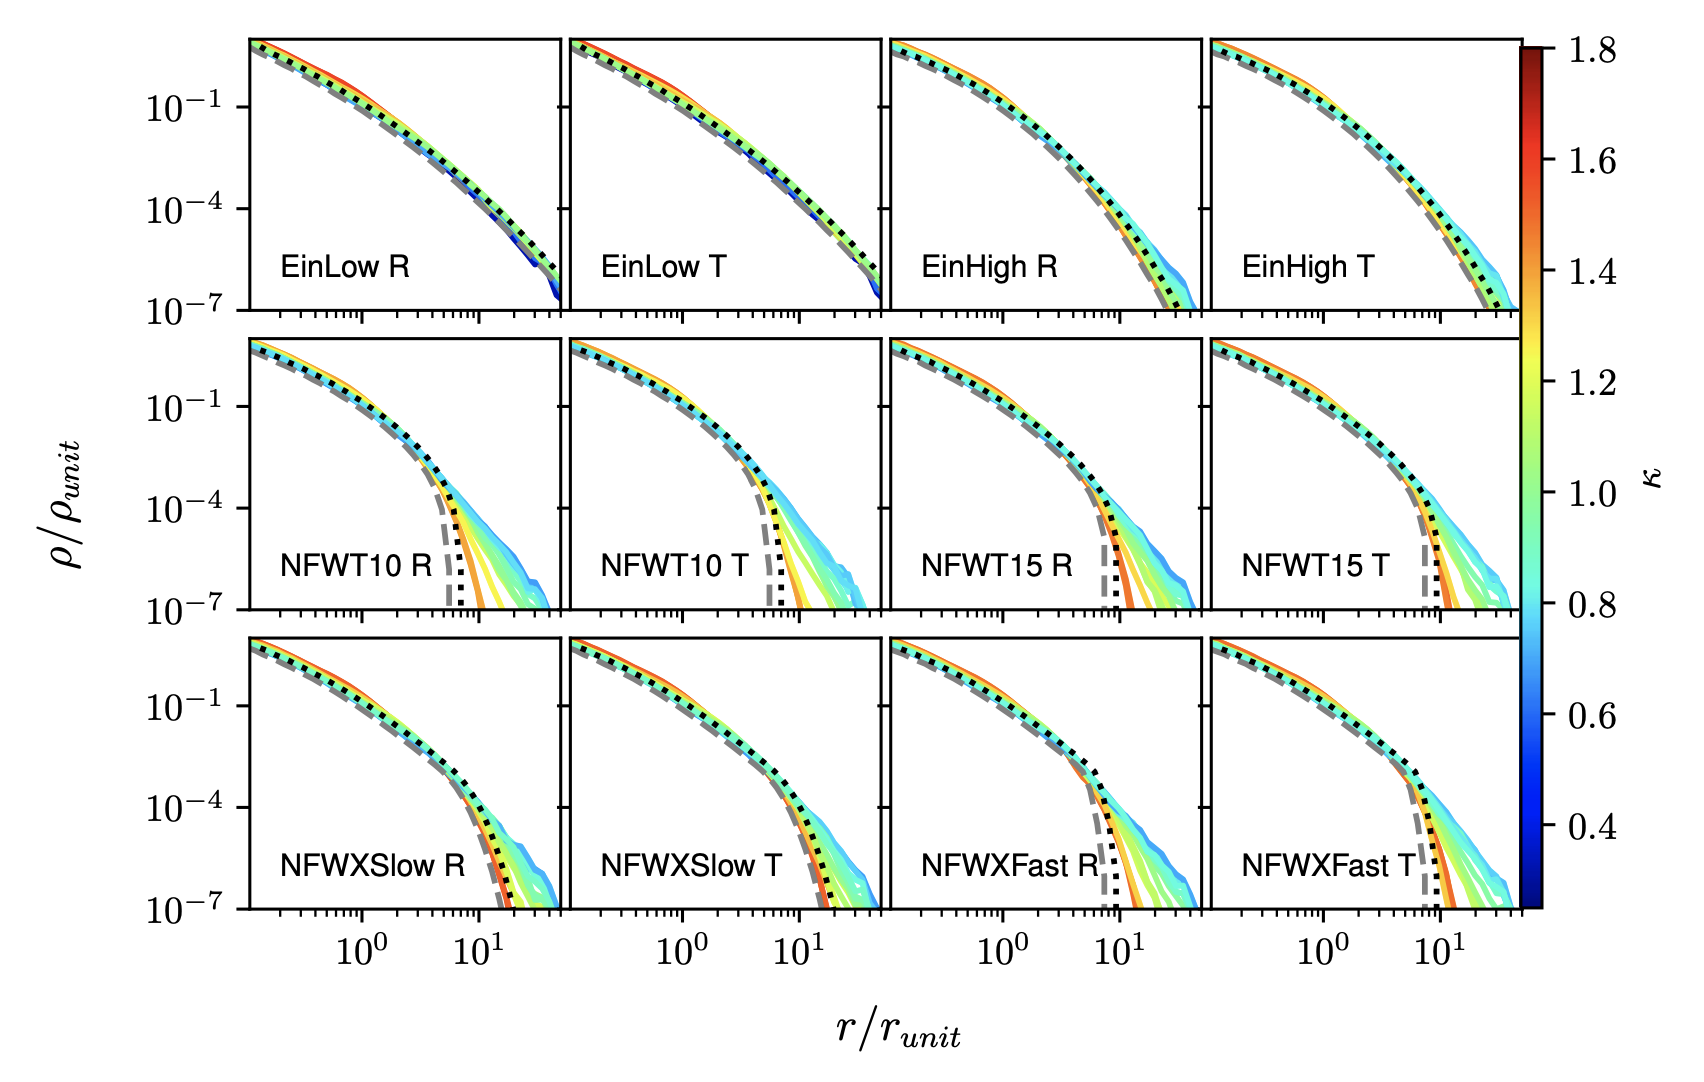
\includegraphics[scale=0.3]{Fig1.png}
\caption{Density profiles of halo remnants for specific initial conditions \citep{Drakos2019II}.}
\label{fig:universe}
\end{figure}


Dark matter is an unknown substance, proposed to only interact gravitationally by Cold Dark Matter (CDM) theories, which is meant to account for the absence of enough visible matter to provide ample gravitational force to bind galaxies together. On large scales, dark matter tends to cluster into filaments, and it is the intersection of these filaments (where the density is higher) that are known as 'halos'. These halos are the exclusive site of galaxy, group, and cluster formation. In order to understand galactic formation and cosmology, an understanding of dark matter halo structure and evolution is essential. \cite{Drakos2019II}.


While some information of dark matter halos can be observationally determined, through means of galaxy kinematics, satellite kinematics, and gravitational lensing, numerical simulation accounts for most of the detailed knowledge of dark matter halos \citep{Drakos2019I}. Halos form in a hierarchical manner, small structures , and also form "inside out", with a bound core collapse with small bits of material becoming loosely bound over time. \cite{Frenk2012}


Despite the basic understanding of dark matter, there are many questions that have yet to be answered, such as:
\begin{itemize}
        \item What is(/are) the fundamental dark matter particle(s) and with what forces does it interact?
        \item How do dark matter halos evolve and form?
        \item What is the underlying structure of all dark matter halos?
\end{itemize}




\section{Proposal} \label{sec:style}


\subsection{Directive} \label{subsec:directive}
The following questions will be addressed:
\begin{itemize}
        \item What is the final density profile ? Is it well fit by a Hernquist profile ? Is it more or less concentrated than the MW or M31 before they merged?
        \item Is the 3D dark matter distribution spheroidal? or elongated like an ellipsoid? What do terms like prolate, oblate, or triaxial halos mean? \citep{Law2009}.
        \item What is the distribution of dark matter particles from the M31 vs the MW?
        \item Where is the ”end” of the halo? How might we define this?
    \end{itemize}
    
\subsection{Approach} \label{subsec:approach}
By simulating the dark matter halo merger under different conditions and in fitting the density profile to known profiles, information about the dark matter halos of the MW-M31 may be discovered.

\subsection{Figures} \label{subsec:figures}
\begin{figure}[h!]
\centering
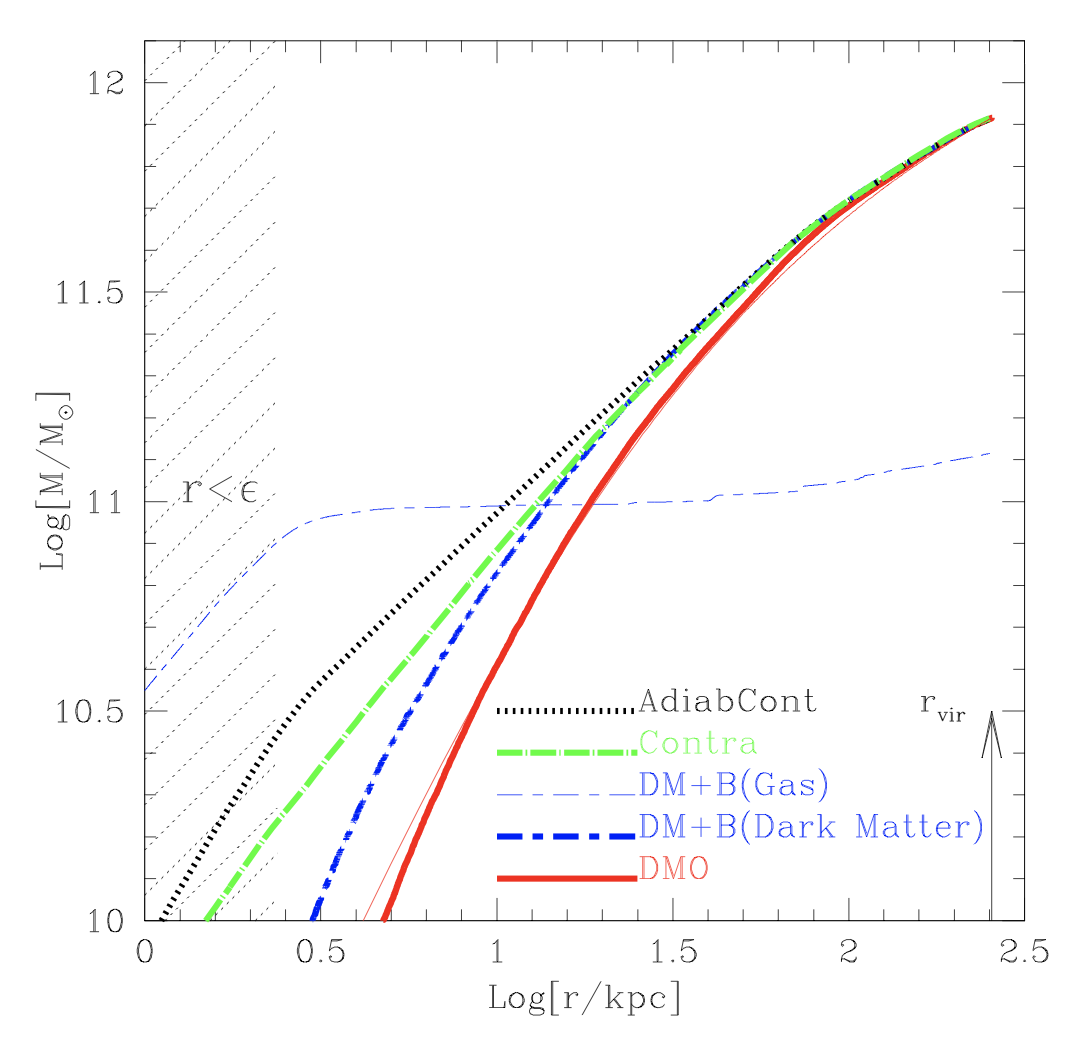
\includegraphics[scale=0.35]{Fig2.png}
\caption{The enclosed mass profile of a certain dark matter halo for specific formulas
\citep{Abadi2010}.}
\label{fig:universe}
\end{figure}

\subsection{Hypothesis} \label{subsec:hypothesis}
I believe that the dark matter halo will have a spheroidal distribution that will fir a Hernquist profile.
\bibliography{ASTR400B_ResearchAssignment2_Lewis}{}
\bibliographystyle{aasjournal}

\end{document}

% End of file `ASTR400B_ResearchAssignment2_Lewis.tex'.